\chapter{Analysis Background}
\label{sec:analysis-background}

This chapter provides a comprehensive background on the analysis of language models, tracing the evolution of methods used to understand transformer architectures and their internal representations. We will cover three main areas: historical approaches to analyzing transformers through attention mechanisms, mechanistic interpretability research, and learning dynamics research. This background will set the foundation for the subsequent chapters that explore specific aspects of language model analysis.

\section{Historical Analysis of Transformers through Attention}

The analysis of transformer architectures has historically centered around understanding the attention mechanism, which serves as the primary mechanism for information flow and representation learning in these models. Early work focused on interpreting attention patterns to understand what linguistic phenomena different components of the model were capturing.

\subsection{Multi-Head Attention Analysis}

One of the foundational studies in transformer analysis was conducted by \citet{voita2019analyzing}, who systematically analyzed the role of individual attention heads in transformer models. Their work revealed that attention heads exhibit specialization, with certain heads becoming interpretable for specific linguistic tasks. For instance, they identified heads that specialized in syntactic dependencies, coreference resolution, and discourse relations. This specialization suggested that transformer models develop a form of modular organization where different components handle distinct aspects of language processing.

The findings of \citet{voita2019analyzing} had practical implications for model optimization. They demonstrated that many attention heads could be pruned without significant performance degradation, as only a subset of heads were actively contributing to the model's linguistic capabilities. This insight supported the development of more efficient transformer architectures through selective head pruning.

Building on this work, \citet{michel2019sixteen} conducted an empirical study that further quantified the redundancy among transformer attention heads. Their analysis revealed that while transformer models are typically trained with multiple attention heads, there is significant overlap in the information captured by different heads. This redundancy suggests that the multi-head mechanism, while theoretically capable of capturing diverse attention patterns, often results in redundant representations in practice.

The work of \citet{michel2019sixteen} provided empirical support for the sparsity hypothesis in transformer architectures, suggesting that many attention heads could be removed or simplified without substantial performance loss. This finding has influenced subsequent research on model compression and efficient transformer architectures.

\subsection{Attention Pattern Analysis in BERT}

\citet{clark2019does} pioneered early methods for analyzing attention patterns in BERT, one of the most influential transformer-based language models. Their work investigated what linguistic phenomena different attention heads were attending to, revealing that BERT's attention mechanism captures both syntactic and semantic relationships.

The analysis revealed that certain attention heads in BERT specialized in syntactic phenomena such as subject-verb agreement, while others focused on semantic relationships like coreference resolution. This specialization suggested that BERT's internal representations encode linguistic structure in a distributed manner across different attention heads.

The methods developed by \citet{clark2019does} for visualizing and interpreting attention patterns have become standard tools in the field of transformer analysis. Their work demonstrated that attention weights could serve as a window into the model's internal decision-making processes, providing insights into how transformer models process and represent linguistic information.

\section{Mechanistic Interpretability Research}

While attention analysis provided initial insights into transformer behavior, the field of mechanistic interpretability has developed more sophisticated methods for understanding the internal representations and computations of language models. This research area focuses on identifying specific neurons, circuits, and mechanisms that implement particular linguistic capabilities, with the ultimate goal of achieving full model interpretability.

\subsection{Foundational Concepts in Mechanistic Interpretability}

The theoretical foundation for mechanistic interpretability was established by \citet{olah2014manifolds}, who introduced the concept that neural networks transform data through layers that continuously deform input spaces while preserving their topology. This work supported the manifold hypothesis, which posits that real-world data lies on lower-dimensional manifolds in high-dimensional input space. This framework provides the mathematical basis for understanding how neural networks, including transformers, organize and transform information through their layers.


\begin{figure}[ht!]
    \centering
    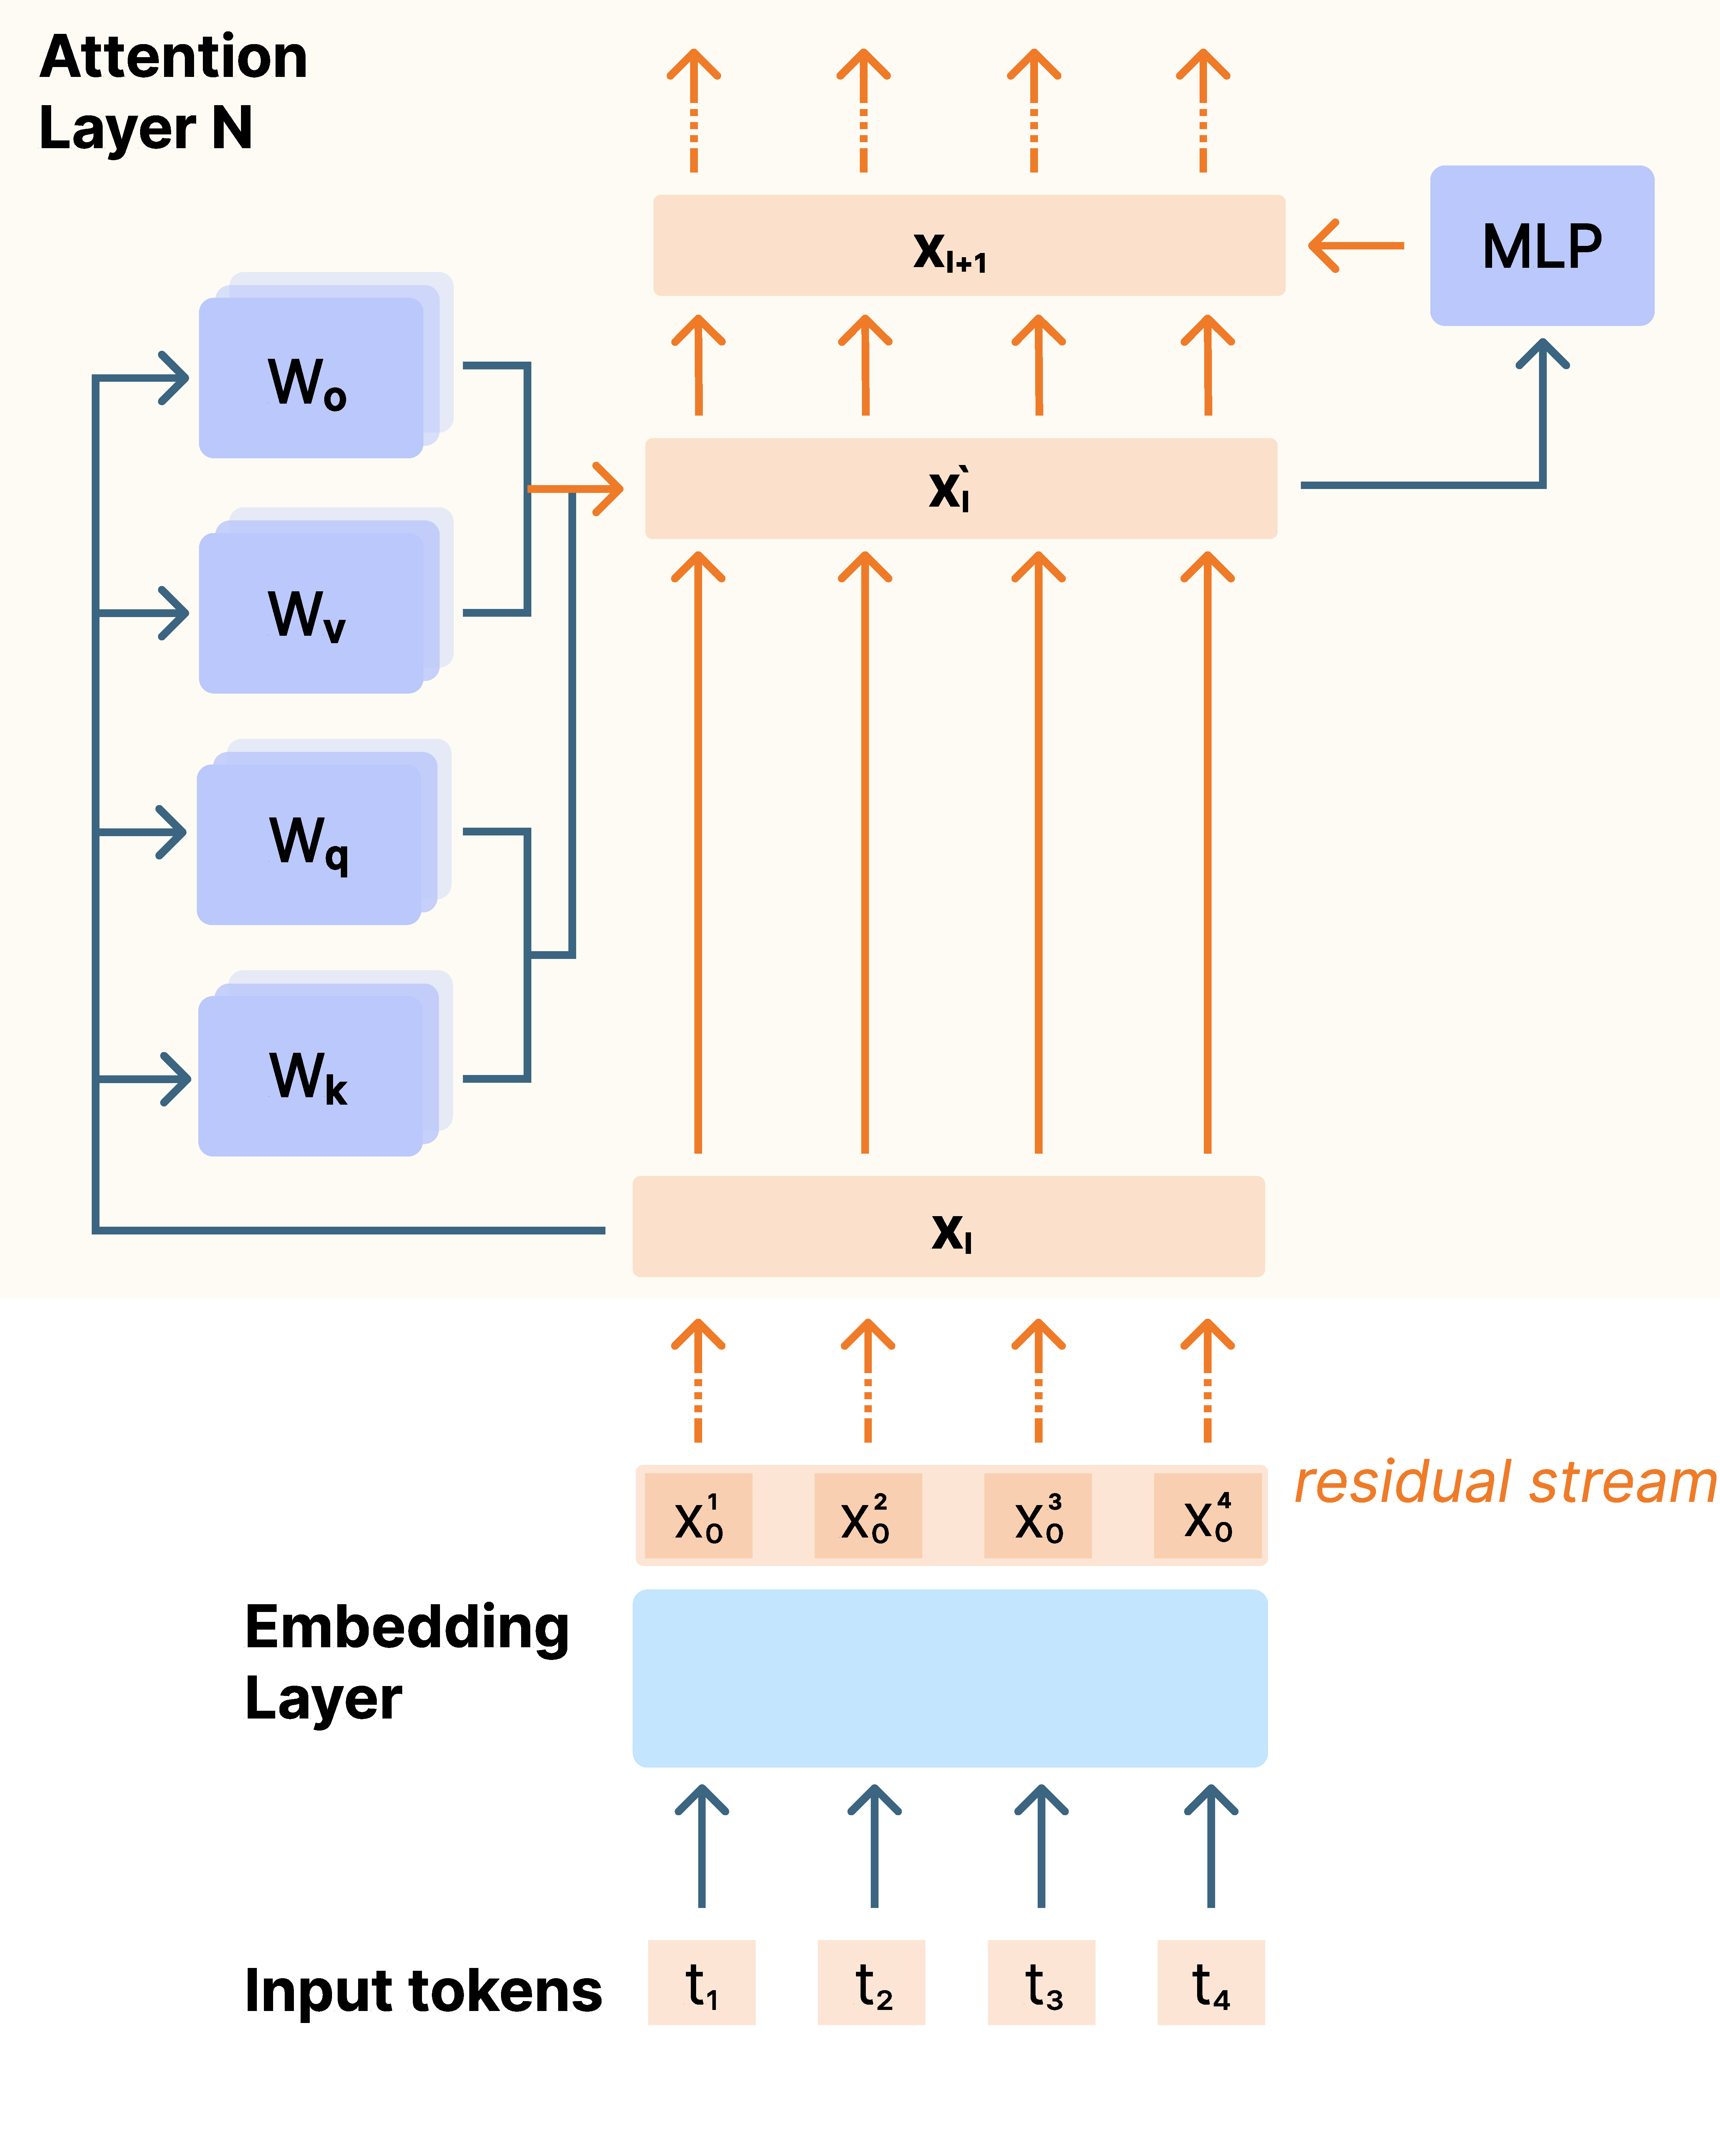
\includegraphics[width=0.6\textwidth]{chapters/analysis_background/figures/residual_stream_visualization.pdf}
    \caption{Visualization of the residual stream in a transformer model, showing how information flows through the network via skip connections and is progressively refined through attention and feed-forward layers.}
    \label{fig:residual-stream}
\end{figure}

\subsection{Circuit-Based Analysis of Transformers}

\citet{elhage2021mathematical} introduced a mathematical framework for understanding transformer architectures through the lens of "circuits" and proposed that transformers can be decomposed into interpretable computational subgraphs. This work developed mathematical tools to analyze attention patterns and their role in computation, showing how attention heads can implement specific algorithms such as copying and induction. The framework introduced the concept of "virtual weights" to explain how attention heads work together, providing a systematic approach to understanding transformer internals.

Building on this circuit-based approach, \citet{olsson2022inductionheads} investigated how transformers perform in-context learning through "induction heads." Their work demonstrated that induction heads are a key mechanism for in-context learning, implementing a specific algorithm for pattern matching. The research provided evidence that induction heads are universal across different transformer architectures and showed how their emergence during training enables various in-context learning behaviors.

\subsection{Superposition and Feature Representation}

\citet{elhage2022toy} introduced a framework for understanding how neural networks represent multiple features in a single neuron through "superposition." This work showed how networks can use superposition to represent more features than dimensions, leading to "interference" between features. The research provided mathematical tools to analyze and understand superposition, demonstrating that it can be both beneficial for efficiency and problematic due to interference. The concept of "sparse coding" was introduced as a way to understand and potentially mitigate superposition effects.

\subsection{Memory Mechanisms in Transformers}

\citet{geva2021memory} proposed that feed-forward layers in transformers act as key-value memory networks. Their work showed that each neuron in the feed-forward layer can be understood as a key-value pair, with these layers storing and retrieving information in a way similar to memory networks. This research provided evidence that feed-forward layers are more important than previously thought and showed how this memory mechanism complements the attention mechanism. The work introduced methods to analyze and interpret the information stored in feed-forward layers.

\subsection{Knowledge Representation and Neurons}

\citet{dai2022knowledge} identified specific neurons in pretrained transformers that encode factual knowledge. Their work showed that these "knowledge neurons" are highly specific to particular facts and that knowledge is distributed across multiple neurons. The research introduced methods to identify and analyze knowledge neurons, demonstrating that they can be used to explain model predictions. The findings provided evidence that knowledge is stored in a way that's both distributed and local, offering insights into how transformers encode factual information.

\subsection{Intermediate Layer Analysis}

\citet{belrose2023eliciting} improved our understanding of how intermediate layers in transformers encode predictive information during generation. Their work generalized the "logit lens" technique by creating a learned diagnostic probe that aligns better with the model's own representations. While the standard logit lens applies the output embedding and softmax to intermediate layer outputs, the tuned lens trains a small set of linear probes to map activations to logits, approximating the final layer's predictions using intermediate activations.

\subsection{Towards Monosemantic Decomposition}

\citet{bircken2023monosemanticity} developed methods for decomposing language models into monosemantic components—neurons or features that correspond to a single, interpretable concept. Their work used dictionary learning (sparse autoencoders) to discover a basis of features from model activations, where each feature corresponds to a sparse, interpretable direction in activation space. The research introduced the concept of monosemanticity, where a component consistently represents one human-understandable feature, and addressed the challenge of superposition where current model activations often mix multiple concepts into a single neuron.

\citet{anthropic2023components} provided a general overview of Anthropic's broader research agenda on mechanistic interpretability, particularly around breaking models into interpretable parts. This work described ongoing efforts toward identifying circuits, features, and neurons that implement human-interpretable behaviors, with the eventual aim of achieving "full model interpretability" where every parameter's role is understood. The research highlighted dictionary learning approaches as promising steps toward faithful model decomposition.

\subsection{Frameworks and Tools for Mechanistic Interpretability}

Several frameworks and tools have been developed to support mechanistic interpretability research. \citet{nanda2022transformerlens} developed TransformerLens, a core library for mechanistic interpretability of transformers that enables detailed inspection of attention heads, MLPs, and circuits. While designed for static model analysis, it provides essential tools for circuit discovery and analysis.

\citet{meng2022locating} introduced ROME, a method for directly editing factual knowledge in transformers. This work built on identifying causal neurons and aligned with post-hoc interpretability approaches, requiring static, trained models for intervention. \citet{conmy2023towards} developed ACDC, which automates the discovery of circuits in transformers using sparse matrix factorization, supporting inference-time interpretability for fixed model weights.

For broader model analysis, \citet{kokhlikyan2020captum} provides a PyTorch library for feature attribution and saliency methods, including Integrated Gradients and DeepLIFT. While less specialized than TransformerLens, it supports a broad class of models and attribution techniques, making it useful for comparative analysis across different architectures.

\subsection{Implications for Language Model Analysis}

The mechanistic interpretability research has profound implications for understanding language models. It reveals that transformers implement sophisticated algorithms through specific circuits and mechanisms, with knowledge distributed across multiple components in ways that balance efficiency with interpretability. The development of tools and frameworks for circuit discovery and analysis has made it possible to systematically investigate the internal workings of these models, moving beyond surface-level attention analysis to deeper understanding of computational mechanisms.

This body of work demonstrates that language models can be decomposed into interpretable components, though the challenge of superposition and the distributed nature of knowledge representation requires sophisticated analysis techniques. The research provides a foundation for developing more interpretable and controllable language models, with applications ranging from model debugging to knowledge editing and safety analysis.

\section{Learning Dynamics Research}

Understanding how language models learn and develop their linguistic capabilities over the course of training has become an important area of research. This work focuses on tracking the emergence of linguistic phenomena during training and understanding the developmental trajectory of language model representations. Learning dynamics research can be broadly categorized into two main approaches: temporal analysis of memorization and influence, and convergence analysis through network similarity measures.

\subsection{Temporal Analysis: Memorization and Influence}

\subsubsection{Influence Functions}

\citet{koh2017understanding} introduced influence functions as a technique from robust statistics to trace model predictions through the learning algorithm and back to training data. This approach identifies training points that are more responsible for a given prediction by perturbing the data input rather than the model itself. The method requires oracle access to gradients and Hessian-vector products, using the result that the influence of upweighting a datapoint on the parameters is given by the inverse Hessian multiplied by the gradient of the empirical risk function with respect to the data point at the current parameters.

Building on this foundation, \citet{grosse2023influence} applied influence functions to large language models to answer counterfactual questions about how model parameters and outputs would change if a given sequence were added to the training set. This work demonstrated the applicability of influence analysis to the scale and complexity of modern language models, providing insights into the relationship between training data and model behavior.

\subsubsection{Forgetting and Memorization Dynamics}

\citet{toneva2019empirical} introduced the concept of forgetting events, tracking when a model flips from correct to incorrect on a given training example during training. This approach provides measures of learning stability and example difficulty, offering insights into the temporal dynamics of learning. While not language-model specific, the methodology has been adapted for NLP applications.

\citet{swayamdipta2020dataset} developed dataset cartography, which measures consistency and variability of model predictions across training epochs. This work applied prediction dynamics to NLP datasets, including BERT fine-tuning, and provided practical applications for understanding dataset characteristics and model learning patterns.

\citet{feldman2020does} explored the memorization-generalization tradeoff using prediction trajectories, discussing example-level dynamics and when memorization is necessary, especially in smaller models. This work provided theoretical insights into the relationship between memorization and generalization in neural networks.

\citet{biderman2023emergent} studied memorization in the Pythia language model family, defining memorization as outputting verbatim training sequences. Their work formulated a forecasting problem: predicting which sequences a large model will memorize using either smaller model runs or early training checkpoints. Key findings included that smaller fully trained models do not reliably predict memorization in larger models, but early checkpoints of the same model do reliably forecast final memorized content, achieving high recall.

\subsection{Convergence Analysis: Network Similarity}

\subsubsection{Canonical Correlation Analysis and Variants}

\citet{raghu2017svcca} introduced Singular Vector Canonical Correlation Analysis (SVCCA), which allows analysis of weight outputs as subspaces without requiring axis alignment. This method enables comparison of representations across different layers and models by analyzing the canonical correlation between their singular vectors.

\citet{morcos2018pwcca} developed PWCCA (Projection-Weighted CCA) to address the noise problem in the original SVCCA approach. They argued that averaging correlations included noise, so instead used a weighted average that rewards signal more heavily when computing the final correlation between singular vectors and original inputs.

\citet{kornblith2019cka} identified limitations of CCA for measuring similarities between representations with higher dimension than the number of data points. They proposed Centered Kernel Alignment (CKA) as an alternative, which learns kernel functions between different inputs to layers of interest and considers how much variance is explained by each input.

\subsubsection{Model Stitching Techniques}

\citet{lenc2015understanding} introduced the concept of stitching layers together in CNNs to reveal structure in the similarity between different layers. This approach provided a new perspective on understanding representation similarity across model architectures.

\citet{bansal2021stitch} formalized model stitching as connecting the bottom layers of one model to the top layers of another with a trainable layer in between. This technique reveals similarity in representations that cannot be captured by CKA and demonstrates that representations trained with more data, larger width, and more training time can improve performance in weaker models.

\subsubsection{Applications to Language Models}

\citet{saphra2019understanding} used SVCCA to show that language model training with ELMo learns similar representations to those of a POS tagger during training, with POS information being learned earlier in the training process.

\citet{nguyen2020wide} used CKA to investigate how neural network representations vary with width and depth. They found that wider and deeper networks develop characteristic block structures in hidden representations, particularly when model capacity is large relative to training set size. These block structures arise when underlying layers preserve and propagate the dominant principal component of their representations.

\citet{singh2019bert} used CCA to demonstrate that multilingual BERT models don't have a universal representation of language. They found that deeper layers diverge in their representations of different languages, with hierarchical clustering revealing tree structures that correspond to phylogenetic relationships.

\citet{phang2021finetuned} used CKA to compare similarity across task-tuned models between layers, finding block structures in the models. They observed that similarity was especially pronounced between later layers, which only marginally contribute to task performance.

\citet{wu2020similarity} analyzed contextual word representation models and found that models in the same family are more similar to one another, while different architectures have similar representations but different individual neurons. This work identified different types of representation similarity across model architectures.

\citet{brown2023understanding} applied metrics like CKA to understand generalization in the Pythia suite, focusing on model comparison post-training rather than training-time convergence. This work emphasized intra-model dynamics during training and provided insights into how different models develop similar or divergent representations.

\subsection{Implications for Language Model Analysis}

The learning dynamics research provides crucial insights into how language models develop their capabilities over time. The temporal analysis approaches reveal the relationship between training data and model behavior, showing how models memorize, forget, and generalize from their training examples. The convergence analysis approaches demonstrate how representations evolve and become similar across different model architectures and training conditions.

These methods enable researchers to track the emergence of linguistic phenomena during training, understand the developmental trajectory of language model representations, and identify the factors that influence model learning and generalization. The combination of temporal and convergence analysis provides a comprehensive framework for understanding language model learning dynamics, with applications ranging from model debugging to curriculum design and interpretability research.
